\setlength{\headheight}{1.2cm}
\renewcommand{\publ}{\flushleft\footnotesize{Based on:\\[0.1cm]
		\textit{D. Sas, P. Avgeriou, Quality attribute trade-offs in the embedded systems industry: an exploratory case study. Software Quality Journal 28, 505-534 (2020). https://doi.org/10.1007/s11219-019-09478-x} \\[0.1cm]
}}

\chapter{Quality attribute trade-offs in the embedded systems industry -- An exploratory case study}
\label{chap:7}
\epigraph{\emph{Reuse is one of the most abused abstractions, because the general view in organizations is that reuse represents a laudable goal that teams should strive for. However, failing to evaluate all the trade-offs associated with reuse can lead to serious problems within architecture.}}{--- Neal Ford, Software Architecture: The Hard Parts}

\begin{Abstract}
    \textbf{\\Context: } The embedded systems domain has grown exponentially over the past years. The industry is forced by the market to rapidly improve and release new products to beat the competition. Frenetic development rhythms thus shape this domain and give rise to several new challenges for software design and development. One of them is dealing with trade-offs between run-time and design-time quality attributes.
    \\\textbf{Objective: } To study practices, processes and tools concerning the management of run-time and design-time quality attributes as well as the trade-offs among them from the perspective of embedded systems software engineers.
    \\\textbf{Method: } An exploratory case study with two qualitative data collection steps, namely interviews and a focus group, involving six different companies from the embedded systems domain with a total of twenty participants.
    \\\textbf{Results: } The interviewed subjects showed a preference for run-time over design-time qualities. Trade-offs between design-time and run-time qualities are very common, but they are often implicit, due to the lack of adequate monitoring tools and practices.
    Practitioners prefer to deal with trade-offs in the most lightweight way possible, by applying ad-hoc practices, thus avoiding any overhead incurred.
    \\\textbf{Conclusions: }
    Although it is notoriously difficult to deal with trade-offs, constantly monitoring the quality attributes of interest with automated tools is key in making explicit and prudent trade-offs and mitigating the risk of incurring technical debt.
\end{Abstract}

\section{Introduction}\label{c7:sec:intro}
Over the past years, embedded systems (ES) have experienced an exponential growth, both in terms of size and complexity as well as the number of domains where they are applied.
However, this growth also brings substantial challenges, one of which is to deal with both the run-time quality attributes that determine system behaviour, and the design-time ones that establish system sustainability.
Managing quality attributes and performing trade-offs between them is notoriously difficult in any field \cite{Bass2012}.
In the case of embedded systems, it is even more challenging, due to the limited hardware resources on which the software is deployed, as well as the rapid evolution of hardware \cite{Mallick2009}. 

The management of trade-offs between run-time qualities on the one side, and design-time qualities on the other, is thus becoming a critical research area. Specifically, the embedded systems industry needs dedicated \textit{tooling}, \textit{processes} and \textit{practices} for managing such trade-offs \cite{Ampatzoglou2016}.
At the moment, several tools are available, both free/open-source and commercial, but only to support the management of \textit{individual} quality attributes of interest in embedded systems.
The management of trade-offs is still an unexplored area: not only there are no tools available, but, to the best of our knowledge, there is also no evidence regarding the specific needs of the embedded systems industry on performing quality attributes trade-offs. 
Thus, this problem can be formulated as a high-level research question: \textit{How are trade-offs between quality attributes currently managed by the ES industry and how can this be improved?} 
%Daily development decisions might have a critical impact on the crucial quality attributes of the project, and thus its final success.

We begin to address this problem through an exploratory case study  investigating how  embedded systems engineers manage trade-offs between run-time and design-time quality attributes and what kind of support they require.
We collected data in three steps. 
First, we performed a series of interviews with eight subjects to obtain a fine-grained understanding of the daily activities they performed and the trade-off decisions they experienced on their projects.
Then, we planned a focus group session with eight subjects (two of them had also taken part in the interviews), discussing the issues, costs, decisions, and related trade-offs of design-time and run-time qualities. The interviewees and the focus group participants worked in five different companies in the embedded systems domain. 
And finally, we interviewed six more participants in order to check, confirm, and possibly extend the findings from the previous two phases.

Our findings shed light on which qualities are prioritised in the studied domain, what kind of trade-offs occur, how these trade-offs take place in practice, and how they should ideally take place. We note that, while our scope encompasses run-time and design-time qualities in general, we pay special attention to  \textit{Maintainability}, \textit{Dependability}, and \textit{Energy Efficiency}. We selected these qualities due to their importance for the embedded systems software development lifecycle \cite{Knight2002,Koopman2004} (further motivation for these 3 qualities is given in Section \ref{c7:sec:objectives-rq}). 

This chapter is organised using the Linear-Analytic Structure version of the case study reporting template proposed by Runeson et al. \cite{Runeson2012}. This template was chosen because it is commonly used to report case studies in Software Engineering.
Section \ref{c7:sec:background} introduces some theoretical background and reports on similar work from literature.
Section \ref{c7:sec:case-study} elaborates on the case study design, while Section \ref{c7:sec:results} reports the results obtained by this work. Section \ref{c7:sec:discussion} presents a discussion on our findings with key take-away messages.
Section \ref{c7:sec:threats} describes some threats to the validity of this study and how they were mitigated.
Section \ref{c7:sec:conclusion} concludes the work presented in this chapter.

\section{Background and Related work}\label{c7:sec:background}
This section summarises the background knowledge necessary to better understand the work presented, and reports on related work.

\subsection{Background and terminology}
The management of the quality attributes of a system is a key activity on which the success of the project and user acceptance heavily depend on.
Indeed, software \textit{quality} is defined as the degree to which software possesses a desired combination of quality attributes \cite{Barbacci1995,IEEE10611992}.

Quality attributes may be categorised according to different criteria; one possible taxonomy is to divide them according to their \textit{run-time} or \textit{design-time} nature \cite{Bass2012}.
The former type includes the quality attributes that describe the behaviour of a system during its execution; in other words, those attributes that impact the usage of the system by external actors, which may be both users or other systems (e.g. Performance, Reliability, Security).
In contrast, design-time quality attributes determine the ease of managing the system artefacts during the software development lifecycle and the sustainability of the system over time (e.g. Maintainability, Reusability, Testability). We adopted such a dichotomy in order to focus our efforts on the trade-offs between the quality attributes across the two categories rather than within them.

As mentioned in Section 1, we pay special attention to  \textit{Maintainability} as a design-time quality and \textit{Dependability} and \textit{Energy-efficiency} as run-time qualities. Maintainability is strongly connected to the concept of \textbf{technical debt} \cite{Kruchten2012}, which plagues all non-trivial embedded systems. Technical debt entails a trade-off (often an implicit one) between the maintainability of a system and  short-term benefits \cite{Kruchten2012}. %\cite{Cunningham1993,Brown2010}
\textit{Dependability} is composed of four sub-qualities, namely \textit{Availability}, \textit{Reliability}, \textit{Safety}, and \textit{Security} \cite{JCLaprie1992}. \textit{Energy efficiency} has become a very prominent run-time quality in the era of the Internet of Things and Cyber-Physical Systems as it affects the battery life of embedded devices \cite{Sherman2008}.

In this chapter, we adopt the definitions of Maintainability, Performance, Interoperability, and Security from ISO/IEC 25010:2011 \cite{ISO25010}. For Reliability we adopt the definition of Fault-tolerance from the standard. Availability is also defined as in the standard, however, we treat it separately from Reliability, while the standard considers it part of Reliability.
For Safety, we adopt the definition provided by IEC 61508-1:2010 \cite{IEC61508}. 

A \textit{trade-off} between two quality attributes is a conscious, or unconscious, decision that positively affects one quality attribute and negatively affects the other.
Trade-offs are an indispensable element of software engineering, as every decision has both benefits and liabilities.
But not every decision may imply a trade-off between quality attributes, and it may not always be the case that the quality attributes involved in a trade-off are explicitly known.
Some decisions may conceal implicit trade-offs which the decision-maker may not be aware of, either at the time of taking the decision or later.
There are several approaches that help to deal with trade-offs; one of the most prominent is ATAM (Architecture Trade-off Analysis Method), which specifically focuses on evaluating the trade-offs while designing, or maintaining, a software architecture \cite{Bass2012,Clements2003}.

\subsection{Related work}
A number of studies provide evidence regarding the trade-offs between run-time and design-time quality attributes in the embedded systems domain.

Ampatzoglou et al. \cite{Ampatzoglou2016} performed an extensive case study on the perception of technical debt in the embedded systems industry, shedding light on how Maintainability is traded-off against other qualities.
A number of engineers from seven companies were interviewed, using a supervised questionnaire-based approach, to elicit information about a total of twenty software components that had accumulated technical debt and were difficult to maintain. 
Their findings show that:
\begin{inlinelist}
    \item Maintainability is more seriously considered when the expected lifetime of the project is over ten years;
    \item the most frequent types of technical debt are test, architectural and code; and
    \item the embedded systems industry prioritises Reliability, Functionality and Performance against Maintainability.
\end{inlinelist}

In a similar context, Wahler et al. \cite{Wahler2017} investigated trade-offs between quality attributes in industrial control and automation systems (ICASs) running on embedded devices.
The authors performed an online survey taken by thirty-seven participants who had worked on real-time embedded systems.
The findings suggest that there are three clusters of qualities that contain positively-related quality attributes.
The first cluster is composed of two run-time qualities -- Timeliness and Predictability -- which means that fulfilling Timeliness eases fulfilling Predictability.
The second cluster is composed of three design-time qualities -- Modularity, Reusability, and Portability -- and again fulfilling one eases fulfilling the others.
The third cluster is composed of a single run-time quality: Efficiency, intended as power consumption and heat dissipation.
The authors state that quality attributes belonging to one of the clusters \textit{negatively influence} the attributes of the others clusters.

Feitosa et al. \cite{Feitosa2015} investigated quality attribute trade-offs among critical and non-critical qualities by analysing twenty open-source Java projects in the embedded software field.
The following findings emerged from their analyses:
\begin{inlinelist}
    \item Correctness negatively affects Performance since solving bugs usually introduces inefficiencies in the source code that affect performance, and
    \item increasing Performance negatively affects Reusability since solutions that improve performance have a negative impact on quality metrics like cohesion, coupling and size.
\end{inlinelist}

Similarly, Papadopoulos et al. \cite{Papadopoulos2018} studied the interrelation between design and runtime quality metrics by examining source code quality and comparing it with the performance and energy consumption of a set of embedded applications.
In their work, they measure source code quality using the Cognitive Complexity metric calculated by SonarQube\footnote{See \url{https://sonarqube.org/}.} and CPU cycles, cache misses, and memory accesses to measure run-time performances.
The authors observed that, by applying certain transformations to the source code of the selected embedded systems, there exist trade-offs between performance/energy consumption and Cognitive Complexity.

A different approach was used by Oliveira et al. \cite{Oliveira2008}, who measured design-time quality metrics on the source code and compared them with performance-related metrics (i.e. memory, time, etc.) measured during the execution of the system.
The authors compared four alternative designs of an example system, showing the existence of trade-offs between design-time quality metrics and performance.
More precisely, the increase of the McCabe Cyclomatic Complexity metric correlated with a decrease in cycles performed and memory used.

A practical approach to managing trade-offs between run-time and design-time qualities was introduced by Corr{\^{e}}a et al. \cite{Correa2010}.
The authors propose an approach for guiding design decisions based on the prediction of physical properties (cycles, power consumption) using traditional software metrics, showing how design decisions impact on the physical properties of the final system.

The work of Mentis et al. \cite{Mentis2009} focuses on evaluating the impact of design decisions on run-time quality aspects for different software architectures (not limited to embedded systems).
Their analysis discovered groups of run-time metrics that strongly correlate among each other, for they were found to be affected by the same architectural factors.
However, their approach is based on simulation data obtained using a tool developed by the authors themselves for a previous study.

Bellomo et al. \cite{Bellomo2015} studied the most common quality attributes that projects must address and their relative importance. 
Their aim was to understand the impact of long-term architectural deterioration (i.e. technical debt) of quality attributes based on quality attribute scenario data generated through the Architecture Trade-Off Analysis Method (ATAM) from multiple projects and multiple domains (including ES) and companies.
Their results show how Modifiability (i.e. Maintainability) is of primary importance in the majority of the projects considered by the study.

Martini et al. \cite{Martini2015} explore, by interviewing fifteen embedded systems practitioners, the input they use to deal with architectural technical debt items caused by non-optimal architectural decisions as well as the priority they attribute to different aspects of software development.
Their findings suggest that Maintainability-related costs are important when prioritising technical debt but they are secondary to other business-oriented factors, such as the competitive advantage.

The presented studies differ from this work in at least one of the following aspects:
\begin{inlinelist}
    \item they base their analyses and conclusions on open-source projects rather than on industrial ones;
    \item they focus on source code analysis rather than on the human factors that caused a particular change in the system;
    \item they do not report on individual trade-off experiences shared by developers.
\end{inlinelist}
We chose these criteria to compare our study to the related work as they comprise the goal of the study and highlight its uniqueness. 
Our study is the only one that fulfils all three of these criteria as summarised by Table \ref{c7:tab:rel-work}.

\begin{table}[!h]
   \footnotesize
    \centering
    \caption{Comparison between related work studies and this study. TO stands for trade-off.}
    \label{c7:tab:rel-work}
    \begin{tabular}{@{}m{5cm}ccc@{}}
    \toprule
    \multicolumn{1}{c}{\textbf{R.W.}} & \multicolumn{1}{c}{\textbf{\begin{tabular}[c]{@{}c@{}}Industrial\\ setting\end{tabular}}} & \multicolumn{1}{c}{\textbf{\begin{tabular}[c]{@{}c@{}}Human\\  factors of TO\end{tabular}}} & \multicolumn{1}{c}{\textbf{\begin{tabular}[c]{@{}c@{}}Report TO\\ experience\end{tabular}}} \\ \midrule
    \cite{Ampatzoglou2016,Wahler2017} & \cmark & \cmark & \xmark \\
    \cite{Bellomo2015,Martini2015} & \cmark & \xmark & \xmark \\
    \cite{Feitosa2015,Papadopoulos2018,Correa2010,Mentis2009} & \xmark & \xmark & \xmark \\ \midrule
    This study & \cmark & \cmark & \cmark \\ \bottomrule
    \end{tabular}
\end{table}

\section{Case study design}\label{c7:sec:case-study}
We followed the guidelines proposed by Runeson et al. \cite{Runeson2012} to conduct and report case studies.
Furthermore, we used the protocol template proposed by Brereton et al. \cite{Brereton2008} to develop the case study design and keep track of its changes. 
The replication package of this study is available online\footnote{Visit \url{http://www.cs.rug.nl/search/uploads/People/repl-package-ds18.zip}. } and includes the case study protocol, the questionnaires of the interviews, the discussion agenda of the focus group, the transcription template, the notes used to explain the technical concept to practitioners, and the consent letter template.
To ensure the quality of the results of this study, we list the threats to validity in Section \ref{c7:sec:threats} and the mitigating actions undertaken to address them.
Moreover, a sanity check of all  results was performed by discussing them in a dedicated meeting of our research group.

\subsection{Objective and Research Questions}\label{c7:sec:objectives-rq}
The objective of this study is made more specific using the Goal-Question-Metric \cite{VanSolingen2002} formulation:
\begin{quote}\textit{
    \textbf{Analyse} the experience of software engineers \textbf{for the purpose} of understanding the management of run-time qualities, design-time qualities and the trade-offs among them \textbf{with respect to} practices, processes and tool support \textbf{from the point of view of} software engineers \textbf{in the context of} industrial embedded system projects.}
\end{quote}

The stated goal leads to four specific research questions:
\begin{description}
    %\item[RQ1] \textit{What are the design-time and run-time quality attributes of interest to the ES industry, and what tools, processes, and practices are adopted to manage them?} Original RQ
    \item[RQ1] \textit{What is the interest of the ES industry in design-time and run-time quality attributes, such as Maintainability, Dependability and Energy efficiency, and what tools, processes, and practices are adopted to manage them?}
\end{description}
This investigates the qualities of interest (in the scope of this study) for practitioners in the ES domain, as well as tools, processes, and practices used to address these qualities individually. We distinguish between design-time and run-time qualities. Once we understand which qualities are of interest, the next question explores their trade-offs. \begin{description}
    \item[RQ2] \textit{What trade-offs between design-time and run-time qualities do ES practitioners make?}
\end{description}
This aims at eliciting knowledge on the compromises and trade-offs between design-time and run-time qualities, as well investigating the \textbf{\textit{implicit}} or \textbf{\textit{explicit}} nature of such trade-offs. Once we understand which trade-offs are made, the next question explores how they are made.
\begin{description}
    \item[RQ3] \textit{What processes, practices, and tools do ES practitioners use to support trade-off decisions?}
\end{description}
This focuses on understanding whether the developers follow processes and practices (formal, ad-hoc or otherwise) for dealing with trade-offs and how these are eventually applied. It is also of interest to check if dedicated or general-purpose tools are used to support the trade-off decision making process. Once we understand how trade-offs are currently made, the next question explores how they should ideally be made.
\begin{description}
    \item[RQ4] \textit{What would be the ideal features of a tool supporting quality attribute trade-off decisions?}
\end{description}
Finally, this research question aims at obtaining insight on the desired features for an ideal tool that supports quality attribute trade-off decisions.
We have chosen to investigate ideal tool support instead of practices or processes because \begin{inlinelist}\item tools are less explored by the current literature \cite{Barney2012}, and\item practitioners urgently need tools to manage trade-offs effectively \cite{Ampatzoglou2016}.\end{inlinelist}

As aforementioned in Section \ref{c7:sec:intro}, qualities of particular interest during this study are:
\begin{inlinelist}\item Maintainability, due to the impact of software maintenance on the overall project costs \cite{Erlikh2000}; \item Dependability, due to its high significance in most embedded systems, especially safety-critical ones \cite{Knight2002}; and \item Energy Efficiency, due to its rising popularity in multiple sub-domains of embedded systems \cite{Koopman2004} \end{inlinelist}.
All of these qualities have a concrete impact on the success of a product in today's embedded systems market as they provide a technological competitive advantage for they affect both costs and end user experience.
While we pay special attention to these three qualities, the study looks at design-time and run-time qualities in general. 

\subsection{Cases, subjects and units of analysis}
The case study was designed as an exploratory embedded multiple-case study \cite{Runeson2012}.
A multiple-case study allows studying multiple cases (each within its own context) with a single protocol.
As shown in Figure \ref{c7:fig:case-study-design}, the companies map to the individual cases (or case subjects) while their domain maps to the context.
Accordingly, the engineers that took part in the study correspond to the individual unit of analysis; thus each engineer represents a single unit.

Table \ref{c7:tab:case-study-subjects} lists the case study subjects along with the application domain of the respective company and the number of engineers involved in the study.

Due to the adoption of two data collection methods, interviews and focus group (described in the next section),  the selection process of the engineers taking part in the study was threefold.
\begin{enumerate}
    \item In the first step, each case subject was asked to designate two or three software engineers to take part in the interviews.
    \item Next, the case subjects were asked to provide, if possible, at least one or two additional engineers to take part in the focus group.
    \item In the third and final step, a second round of interviews was performed interviewing a different set of engineers.
\end{enumerate}

This process of data collection ensured \textit{data source triangulation} (i.e. collecting the same data at different occasions) and \textit{methodological triangulation} (i.e. combining different types of data collection methods) \cite{Runeson2012}.

Overall, \textit{\textbf{twenty engineers}} with experience ranging from one to thirty years, working in six different companies, took part in the study.

\begin{figure}
    \centering
    %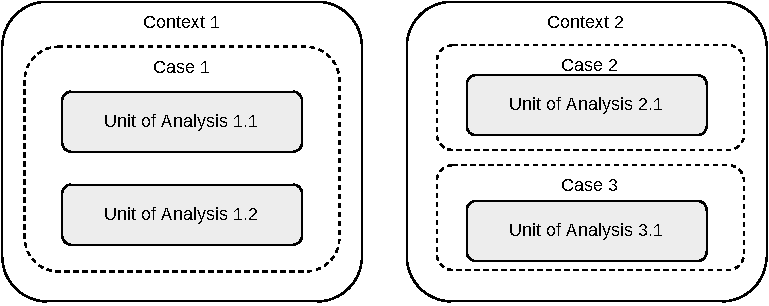
\includegraphics[width=0.8\textwidth]{c7/case-study-design}
    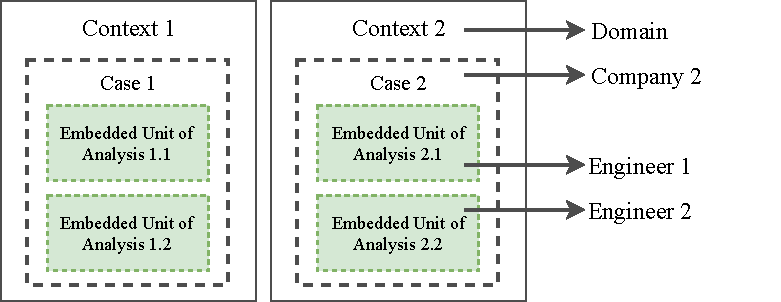
\includegraphics[width=0.8\textwidth]{c7/Fig1.pdf}
    \caption{Embedded multiple-case study design; based on Figure 3.1 by Runeson et al. \cite{Runeson2012}.}
    \label{c7:fig:case-study-design}
\end{figure}

\begin{table}[tbp]
    \centering
   \footnotesize
    \caption{The case study subjects. Size classification follows European Union's SME classification based on the number of employees: Small ($< 50$), Medium ($< 250$), Large ($\ge 250$).}
    \label{c7:tab:case-study-subjects}
    \begin{tabular}{@{}cllc@{}}
    \toprule
    \multicolumn{1}{c}{\textbf{Case subject}} & \multicolumn{1}{c}{\textbf{Domain}} & \textbf{Size} & \textbf{\# of Engineers} \\ \midrule
    C1 & Defense and civil aviation & Large & 6 \\
    C2 & Industrial wearables & Small & 4 \\
    C3 & High Performance Computing & Medium & 3 \\
    C4 & Medical implants \& HPC & Small & 4 \\
    C5 & Automotive & Large & 1 \\
    C6 & IoT \& Sustainable Energy & Medium & 2 \\\midrule
    \multicolumn{3}{l}{\textit{\textbf{Total}}} & 20 \\\bottomrule
    \end{tabular}
\end{table}

\subsection{Data collection}
The research questions were explored by collecting \textit{qualitative data} through a series of individual \textit{interviews} and a \textit{focus group}. 
The following subsections describe both data collection methods in more detail.

\subsubsection{Interviews}\label{c7:sec:interviews}
Interviews were designed following a semi-structured format, composed of a set of predefined open questions, with the possibility for the interviewer to further investigate interesting answers, and for the interviewee, to freely elaborate on them.
The questionnaire can be found in the replication package\footnote{Visit \url{http://www.cs.rug.nl/search/uploads/People/repl-package-ds18.zip}. }.

Before the interviews began, practitioners were asked to think of a \textit{brownfield} project on which they had worked on for at least one year and which had at least two of the following quality attributes among their key drivers: \begin{inlinelist}  \item \textbf{Maintainability} (i.e. technical debt), \item \textbf{Dependability} (Availability, Reliability, Security and Safety) and \item \textbf{Energy Efficiency}.\end{inlinelist}
Such a request was necessary in order to guarantee that the subjects were referring to a project that had had enough time to accumulate technical debt and was concerned with the quality attributes of interest to this study.
More specifically, brownfield projects have an inherent amount of accumulated technical debt, whereas greenfield projects do not have big maintenance issues.
Additionally, working on a project for at least one year increases the knowledge of the system, allowing the practitioner to obtain a deep understanding and experience.

Interviews were performed in two rounds spanning one year one from the other but following the same protocol and questionnaire (strengthening data source triangulation \cite{Runeson2012}). In the first round, eight interviews were performed, whereas in the second, six.
Background details on the fourteen interviewed practitioners and the related projects is reported in Table \ref{c7:tab:iw-participants-background}. The participants were interviewed through video-conferencing for approximately one hour each. 
Prior to performing the actual interviews, two pilot interviews were performed to calibrate the case study protocol and particularly to refine the questions. The first pilot suggested that there was a lack of clarity in some of the questions, and that an initial written list of the topics covered by the interview was necessary to allow the practitioners to prepare themselves upfront.
The change required updating the protocol, which prevented us using data from the first pilot in the analysis phase.
Concerning the second pilot, the interview allowed us to improve the time required to ask the interviewee all the questions and it did not result in any change to the protocol.
Although minor changes to the questions were made, none of them was enough to impact the validity of the interview. Hence, the data from the second pilot interview was considered valid and was used in the analysis.

Each interview spanned five phases: the first and the last correspond to the introduction and the conclusion phases respectively, while the other phases were dedicated to data collection, as can be seen in Figure \ref{c7:fig:interview-phases}.
After transcribing the recordings, each transcription was reviewed by the interviewee in order to avoid misunderstandings.

Concerning the projects discussed with the fourteen interviewees, two of them talked about the same project, thus thirteen projects were analysed in this study.
Finally, all interviewees gave their explicit permission for their interview to be recorded.

\begin{table}[tbp]
   \footnotesize
    \centering
    \caption{Background information on the interviewee and their respective projects.}
    \label{c7:tab:iw-participants-background}
    \begin{tabular}{@{}cc>{\centering\arraybackslash}m{2.5cm}>{\centering\arraybackslash}m{1.5cm}>{\centering\arraybackslash}m{1.5cm}cc@{}}
        \toprule
        \multirow{2}{*}{\bfseries ID} & \multirow{2}{*}{\bfseries Comp.} & \multirow{2}{*}{\bfseries Project} & \multirow{2}{*}{\bfseries Platform} &\multirow{2}{*}{\shortstack{\bfseries Role in \\ \bfseries the comp.}} & \multicolumn{2}{c}{\bfseries Years of exp.} \\
        &  &  &  &  &\multicolumn{1}{c|}{\bfseries curr. role} & \textbf{in total} \\ \midrule
        I1 & C1 & Onboard airborne surveillance system & C++, WinXP  & Software Engineer & 2 & 17 \\
        I2 & C1 & Onboard airborne surveillance system & C++, WinXP  & Software Engineer & 10 & 16 \\
        I3 & C1 & Black box software for UAV drones & C++  & Software Architect & 8 & 13 \\
        I4 & C1 & UAV patrol drone & C++  & Software Architect & 2 & 2\\
        I5 & C2 & Meteorological station with distributed sensors & Java  & Software Architect & 5 & 11 \\
        I6 & C2 & Smart Glasses for industrial technical assistance & Java & Software Engineer & 3 & 7 \\
        I7 & C3 & Quantum Chromodynamics computations & Java + VHDL & Application developer & 3 & 3 \\
        I8 & C3 & Scientific calculations on FPGAs & Java + VHDL & Application developer & 1 & 2 \\
        I9 & C4 & Framework for brain simulations on FPGA & Java + VHDL & Application developer & 6 & 6 \\
        I10 & C4 & Security-by-design for IMD & C + VHDL & Application developer & 2 & 7 \\
        I11 & C4 & Object tracking application on FPGA & C + VHDL & Application developer & 2 & 2 \\
        I12 & C2 & Smart Glasses for industrial technical assistance & Java & Software Engineer & 7 & 10 \\
        I14 & C6 & Distributed mobile sensing platform & C++ & Software Engineer & 1 & 1 \\
        I15 & C6 & Network of power meters for solar panels & Python, Raspberry Pi & Software Architect & 6 & 6 \\
        \midrule\midrule
    \multicolumn{5}{l}{\textit{\textbf{Average}}} & 4.1 & 7.3 \\ \bottomrule
    \end{tabular}
\end{table}
\begin{figure}
    \centering
    % \includegraphics[width=0.95\textwidth]{c7/interview-phases}
    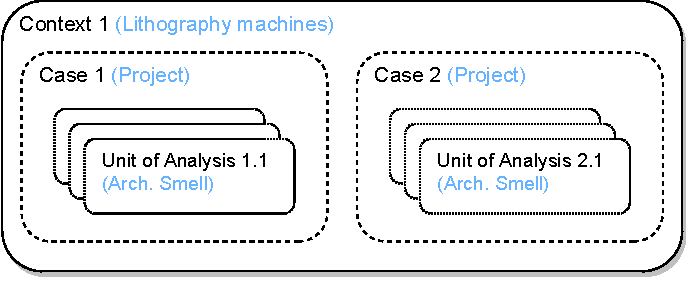
\includegraphics[width=0.95\textwidth]{c7/Fig2}
    \caption{The format of the interviews.}\label{c7:fig:interview-phases}
\end{figure}

\subsubsection{Focus group}
% Description of the FG procedures
The focus group session was performed for the purpose of \emph{triangulating} the results with the data from the interviews (methodological triangulation \cite{Runeson2012}).
Additionally, the focus group enriched the findings from the interviews and explored, from a \emph{group viewpoint}, the practices adopted by the subjects in real-world embedded system projects.
The focus group guide can be found in the replication package\footnote{Visit \url{http://www.cs.rug.nl/search/uploads/People/repl-package-ds18.zip}. }.

It is important to note that, in a group setting, subjects express more explicit and detailed views about their needs due to cognitive mechanisms that activate only through active discussion with other subjects similar to them \cite{Mcdonagh2000,Kontio2008}. Moreover, during a focus group, practitioners can also compare their experience with the other participants and provide unbiased feedback (to the other group members) from an extraneous point of view.
Hence, by pairing the focus group with a number of individual interviews, we collected both personal experiences and group opinions. 

In total, eight participants were involved in the focus group; two of them had also taken part in the interviews.
The session was guided by the two co-authors, fulfilling the assistant and moderator roles respectively, as suggested by Kontio \cite{Kontio2008} and McDonagh-Philip \cite{Mcdonagh2000}.
The format adopted for this data collection step was semi-structured and divided into phases, as depicted in Figure \ref{c7:fig:focus-group-phases}.
After introducing the participants to the focus group dynamics, background information about the participants was collected and is reported in Table \ref{c7:tab:fg-participants-background}.
Contrary to what we did during the interviews, we did not ask practitioners to focus on a single project, but rather we deliberately let them talk about their whole experience in the industry. This choice simplified the session, as it would have been impractical and too time-consuming to ask each participant to select a project and share a minimum amount of context with the other participants in order for the discussion to make sense.
Next, the conversation continued with the main discussion points, prepared prior to the beginning of the session, that touched upon the same topics, and in the same order, as the ones from the interviews. 
The session ended after 1 hour and 45 minutes and was recorded and transcribed with the consent of the participants.

Prior to the beginning of the focus group, the participants had also received a brief written introduction with some examples explaining the technical terminology adopted throughout the discussion.
This succinct explanation prepared them for the beginning of the session, whereas the introduction phase covered any other gaps in their theoretical knowledge.
The discussion points were designed in a semi-structured way and focused on trade-off decision making and related support, since the data collected on these topics during the interviews needed to be further strengthened by the focus group.
Specifically, they first covered the three main quality attributes of this study (i.e. Maintainability, Dependability, Energy Efficiency) in order to initiate the technical discussion.
Then, the discussion moved to implicit and explicit trade-off experiences and related opinions.
In the end, ideas on an envisioned tool supporting trade-offs management were proposed and discussed by the participants.
The contribution of each participant in the discussion was overall balanced.
Nonetheless, two of the participants made fewer interventions than the average did, whereas another one intervened in most of the discussions and required the intervention of the moderator.
Moreover, two factors, namely the semi-structured format of the focus group and the presence of two moderators, ensured that the discussion had a specific direction at any point and that the two participants (out of eight) that were also interviewed did not unveil details that would bias discussion and the other participants.


\begin{figure}
    \centering
    % \includegraphics[width=0.80\textwidth]{c7/focus-group-phases}
    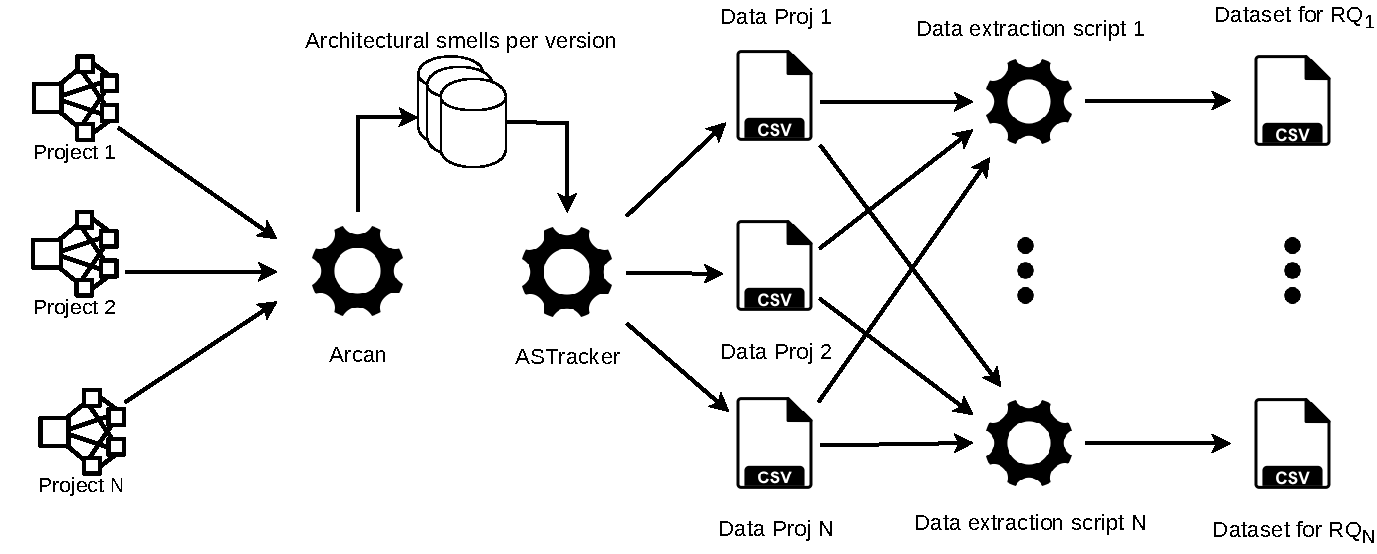
\includegraphics[width=0.80\textwidth]{c7/Fig3}
    \caption{The format of the focus group.}\label{c7:fig:focus-group-phases}
\end{figure}

\begin{table}[tbp]
   \footnotesize
    \centering
    \caption{Background information of the focus group participants, including the typical project size these practitioners work on. * denotes subjects that were also interviewed.}
    \label{c7:tab:fg-participants-background}
    \begin{tabular}{@{}cccc>{\centering\arraybackslash}m{2cm}cc@{}}
    \toprule
    \multirow{2}{*}{\textbf{ID}} & \multirow{2}{*}{\textbf{Company}} & \multicolumn{2}{c}{\textbf{Typical project size}} & \multirow{2}{*}{\bfseries\shortstack{Role in \\the company}} & \multicolumn{2}{c}{\textbf{Years of exp.}} \\
            &  & \multicolumn{1}{c|}{\textbf{in SLOC}} & \textbf{in PM} & \multicolumn{1}{c}{} & \multicolumn{1}{c|}{\textbf{curr. role}} & \textbf{in total} \\ \midrule
    P1 & C1 & 1,000,000+ & 15-100 & Key Account Manager & 13 & 31 \\
    P2 & C1 & 50,000+ & 4 & System Architect & 15 & 22 \\
    P3* & C2 & 10,000+ & 3 & Software Architect & 5 & 11 \\
    P4* & C2 & 10,000+ & 3 & Software Engineer & 3 & 7 \\
    P5 & C2 & 10,000+ & 3 & CEO & 5 & 17 \\
    P6 & C3 & N/A & 6 & Project and Research Manager & 3 & 5 \\ 
    P7 & C4 & 15,000 & 80 & Chief Engineer & 10 & 15 \\
    P8 & C5 & 500,000+ & 7 & Project Manager & 2 & 12 \\ \midrule\midrule
    \multicolumn{5}{l}{\textbf{\textit{Average}}} & 7 & 15 \\ \bottomrule
    \end{tabular}
\end{table}

\subsection{Data analysis}
% Analysis procedure
The analysis of the interviews was performed using the Constant Comparative Method (CCM) \cite{Boeije2002} (which is part of Grounded Theory \cite{Glaser1968}), with the support of a dedicated software tool for qualitative data analysis, Atlas.ti\footnote{See \url{https://atlasti.com}.}.
Grounded Theory (GT) was used because it is one of the most important methods in the field of qualitative data analysis and it has been used extensively within both social sciences and software engineering.
Additionally, GT provides a structured approach to analyse and process the data collected from multiple sources, causing the theoretical sensitivity of the researcher to grow as the data analysis progresses and eventually allow him to formulate hypotheses and theory.

During data analysis, the CCM allowed us to better understand the data and identify links between separate data points by comparing the differences and similarities (using Atlas.ti's features in addition to simple tables and diagrams) within a single interview, between interviews of the same case, interviews from different cases, and between interviews and statements from the focus group.
The analysis started by coding the available data using special keywords, like ``trade-off'' and ``quality attribute'', as codes.
The coded quotations (i.e. the excerpts associated with a code) were also linked, whenever necessary, using links of different types (\textit{continued by}, \textit{criticises}, \textit{justifies}, etc.), provided by default by Atlas.ti.
Following the guidelines of Runeson et al. \cite{Runeson2012} for analysing qualitative data, during the analysis, we continuously added new codes when necessary, updated the existing ones and organised the final forty-nine codes by group.
Additionally, we also created a labelled network, available in the replication package, highlighting the relations between the codes.
Next, thanks to such an organisation of the codes and quotations, we were able to query the data, summarise the information, and fill it into tables used to compare related concepts and experiences among the participants or among the different interview phases. 
Interesting findings and conclusions were eventually inferred and annotated separately.
The process was iterative and was repeated several times until no new findings emerged from the analysis.

For the purpose of better understanding the analysis process, let us suppose we wanted to know what practitioners think of Maintainability. 
To do so, we queried, through Atlas.ti, all the coded statements related to the group of codes "Maintainability". Next we started reading all the statements, compared the opinions in order to understand the differences or similarities, and then summarised with own words their opinion in dedicated tables.
The tables had as rows the quality attributes of interest and as columns the interviewee ID, plus a general column describing the general opinion.
These entries were updated and revised with each iteration of the analysis process.

Special attention was drawn to create a chain of evidence between the final results, the intermediary data structures, and the interview transcripts.
Chains of evidence allow tracing back the origin of a particular piece of information to its original source in case a review of the results might be necessary for the future.

The same methodology -- CCM -- was adopted for analysing the data from the focus group.
The recordings allowed us to easily discern the exact participant contributing to the discussion, whereas the same tables and diagrams were adopted to compare and contextualise the different statements of each participant.

\section{Results}\label{c7:sec:results}
The following sub-sections report on the findings of this study, organised per research question.

Before presenting the results, it is noteworthy to mention that the data collected amounts to fourteen hours of recordings (almost thirteen hours of interviews, counting an average of 50 minutes on average per interview, and one hour and forty-five minutes of focus group).

The results from RQ1 are mostly based on the interviews and partially triangulated by the focus group.

The results from RQ2 are more mixed and contain one example (number 4) exclusively mentioned in the focus group, one example (number 3) coming from the interviews but mentioned by multiple focus group participants, and the rest come from the interviews exclusively.

Concerning instead RQ3, it is hard to determine a precise contribution as both interviewees and focus group participants were sharing similar opinions and experiences.

Finally, the features mentioned by practitioners in RQ4 are equally split between focus group and interviews: three features were mentioned both in interviews and focus group; three were exclusively mentioned in the focus group whereas four were exclusively mentioned in the interviews.
It is interesting to note that only few minutes of focus group managed to produce a comparable number of ideal features as fourteen individual interviews, showing how group dynamics enable creative thinking.

\subsection{RQ1 -- What is the interest of the ES industry in design-time and run-time quality attributes,  such  as  Maintainability,  Dependability  and  Energy  efficiency,  and what tools, processes, and practices are adopted to manage them?}
To understand which quality attributes are the most important, we explicitly asked practitioners to discuss and rank the quality attributes of interest in their projects.
We provide next some qualitative details on the quality attributes of interest alongside the description of the tools, processes and practices used by the practitioners for each quality attribute.
We start with run-time quality attributes:
\begin{itemize}
    \item \textbf{Dependability} includes Availability, Reliability, Security, and Safety, with the first two being the highest priority in general. Availability and Reliability are intrinsically dependent on each other and this aspect is reflected by the fact that the same practices, such as software testing, flight simulations, flight tests, and test-benches with simulated sensors, are adopted to enforce both of them.
    There are also cases where not only Reliability and Availability are highly connected, but also Safety, like in the case of flying drones, where the inability to send commands to a drone could result in dangerous situations.
    Let us discuss each sub-quality attribute separately:
    \begin{enumerate}[label=\alph*)]
        \item \textbf{Availability} is safeguarded using different techniques, depending on the domain of the project, such as: performance measurements with different tooling, static analysis tools for bug identification (i.e. Coverity\footnote{See \url{https://scan.coverity.com/}.}), test benches with simulated hardware, flight simulators, and log inspection for pinpointing issues not identified automatically. In the case of the medical project, it adopted multiple state-of-the-art design principles to ensure no compromises over this quality, like for example intentionally allowing an unlimited number of authentication attempts to the implant device and exploiting energy harvesting techniques to ensure the device does not consume all the battery while processing them. Another example, was the offloading of all the operations related to Security on a separate processor, so that the main one is completely free to perform a specific medical task.
        
        \item \textbf{Reliability} is closely related to Availability, so similar techniques and tools are used to measure and assess its level.
        There were also cases were Reliability (on its own) was a critical quality attribute and special measures were adopted to enforce the quality. For example, in one case the failure of a small percentage (of thousands) of remote sensors could have a big impact on the company's business; hence a sophisticated logging system was developed in order to monitor, detect, classify, and report every failure and facilitate a root cause analysis of the problem.
        In another case, the subjects prepared a special test to ensure the reliability of the connectivity of the system in extreme conditions, and live-tested the product in conditions that it was not originally designed to work in. 
        The term Robustness was also used by some of the subjects with the same meaning as Reliability (they used both terms interchangeably).

        \item \textbf{Security} was of secondary importance, since most of the projects did not manage any sensitive data.
        Among the projects that did have security-oriented components, very few of them employed tools (e.g. BurpSuite\footnote{See \url{https://portswigger.net/burp}.}) to statically check the code to identify possible vulnerabilities.
        In the case of medical devices, were Safety is at risk if the Security of the device is at risk, developers considered using verification tools and provers (such as Tamarin Prover\footnote{See \url{https://tamarin-prover.github.io/}.}, or AVISPA\footnote{See \url{http://www.avispa-project.org/}.}) to check their implementation of the ISO 9798 standard, however, they deemed it was not necessary for such a simple protocol.
        As a final note, there was also a case were neither encryption, nor any other security measure, was considered even though the project involved data exchange over the network; this in contrast to common practices.

        \item \textbf{Safety} was not a major concern in most of the projects, as they did not have to perform safety-critical operations.
        However, two of the projects were safety-critical, and in those cases safety was strictly tied with other qualities, such as Availability, Reliability, Security and Energy efficiency.
        For example, in the medical implant project, where Safety is their mantra, all four of these qualities were necessary to be guaranteed in order to achieve the expected level of Safety from an implantable medical device (IMD).
        Generally speaking, the interviewed practitioners, to enforce Safety, employed techniques such as state-of-the-art design principles (such as the ones mentioned for Availability), flight simulations, intense testing and real-world flying tests. 
        
    \end{enumerate}
    According to the comments of some of the interviewees, Security and Safety were the least prioritised. This fact is because, at the beginning of a project, it is first more important to achieve a high level of Availability and Reliability to be able to impress the management and the eventual customers. Thus, they pay extra attention to such quality attributes first (namely, they \textit{prioritise} them), and then, later on, before delivering the product to the customer, they focus on meeting all the Security and Safety requirements of the specific domain the customer is operating in.
    This can be seen as a prioritisation w.r.t time, rather than importance, i.e. Security and Safety are carefully taken care of at a later stage and certainly before delivery.

    Before moving on to the next quality attribute, we present, as an example, how the results on this quality attribute were obtained through the chain of evidence.
    The first piece of evidence is encountered in the coded data, where Dependability had its own dedicated code (along with four children codes, for its four sub-qualities). Next, all the Dependability-coded data was summarised in a structured table that included also the other quality attributes. Since the reporting is based on such tables, the chain of evidence, from reporting to raw-data, is complete.

    \item \textbf{Energy Efficiency} at the software level was not at the top of the priorities in the projects studied.
    On the other hand, energy efficient hardware and hardware design were deemed much more important and prioritised.
    In many cases, the main source of energy consumption was located in the hardware parts (i.e. motors) or in the design of the hardware itself (e.g. FPGA and IMD design), mostly ignoring the software part.
    At the software level, the most common practice used to assess energy consumption is monitoring the computational resources used by the software (CPU, memory, network, disk, etc.) or used by the hardware managed by the software (e.g. sensors misuse).
    A similar case, where resource usage and energy consumption are strictly tied, is when a cloud back-end is required to manage the IoT infrastructure of the system. In this case, practitioners saw the costs generated by the cloud back-end as energy-related costs that critically impacted the business, and they used the tools made available by the cloud service to guide their energy refactorings. 
    
    Finally, it is interesting to report that in one project, after a year of development, it turned out that the intensive resource usage and sensor misuse were causing excessive energy usage, which, along with severe architectural issues, resulted in a complete rewrite of the system.

    
    \item \textbf{Performance} is especially important in HPC projects, where it is the main driver for every decision made, practice and tool employed (especially at the hardware level).
    Regarding embedded projects, it is not of high priority, as it mostly depends on the projects needs rather that having explicit performance requirements imposed by the needs of the domain.
    Concerning the tools and practices used to measure and monitor performance, two approaches were mentioned often.
    The first one is the plain inspection of the logged timestamps, while the second one relies on dedicated tooling (such as VerySleepy\footnote{See \url{http://codersnotes.com/sleepy/}.}, or built-in functions when available) to profile the execution time of the CPU (and other resources).
    In general, \textit{resource usage} is one of the key aspects of decision making for speed, general optimisations and other decisions.
\end{itemize}

Concerning design-time qualities, we observed the following:
\begin{itemize}
    \item \textbf{Maintainability} was a crucial aspect in most of the projects discussed.
    However, no team reported using dedicated tools to measure and manage it, despite having to deal in most case with issues, such as code duplication and magic numbers, that are easily detectable by modern tools.
    In fact, some projects had experienced major maintainability issues due to accumulation of technical debt; in one case, this eventually caused the bankruptcy of the project \cite{Ampatzoglou2015}, forcing the team to rewrite the system from scratch.
 
    The most commonly-mentioned arguments for striving for high maintainability include the addition of new members to the team (which may substitute existing ones), the architectural complexity of some parts of the system (that need to be easily understood despite their complexity), and the necessity to support future changes, both at software and hardware level, not through trial-and-error but by-design. 
    Contrary to Dependability, Maintainability, despite being \textbf{\textit{deemed}} very important, it is often \textbf{\textit{down-prioritized}} in practice as it is an easy target for cutting corners (prioritisation w.r.t importance).
    
    Some subjects mentioned certain programming practices that they follow in order to increase Maintainability, such as coding rules, conventions, applying design patterns, and common sense.
    Other subjects, from company C1, explained how they employ documentation to transfer knowledge between teams and from old projects to new projects, especially because the developers working on those projects change very often (every 6 months on average). 
    That company works in the aviation sector, which is safety-critical, thus they rely on source code comments and documentation to keep track of every hack and optimisation made in the code. The documentation is then inspected every time the code is transferred to new projects to be reused to ensure that such hacks and optimisations do not cause any issues in the new project.
        
    Lastly, it is worth mentioning that some sub-qualities of Maintainability mentioned by the subjects are Modularity, Readability, Flexibility, Reusability and Understandability. None of them is monitored or measured in any way, similarly as mentioned above for Maintainability. 
    
    \item \textbf{Extensibility} plays an important role in many of the studied projects since new functionality, new sensors, and new hardware in general, are required to be added to the systems with minimal effort, and, in some cases, without stopping the system.
    As in the case of Maintainability, several subjects stated that they do not use any tool to measure or monitor this quality, but they specifically address it up-front during design-time (at an architectural level).

    \item The \textbf{ease of deployment} (Deployability) on multiple platforms is a quality attribute that is important only for certain types of projects.
    Specifically, some companies need to deploy off-the-shelf systems on arbitrary hardware (e.g. drones, FPGA), rapidly adapt them to the new hardware platform and extend them with custom modules specialised for the specific tasks required by the customer.
    A tool-chain developed in-house is used to automate the whole process.
    
    In another company, the continuous change forced by rapid technology advancements (every 6 months), and the high competition in the sector, require continuous hardware upgrades in order for the company to remain competitive.
    In such a scenario, the subject's strategy was to keep the project’s source code as independent as possible from the platform on which it is deployed on, so every time the hardware changes, the changes in the software are minimised.

    \item \textbf{System interoperability} was also addressed by some of the subjects in order to make the system compatible with several types of sensors for data collection, receiving input from controlling devices and sending data streams to different devices (e.g. smartphones, central control stations).
\end{itemize}

\subsection{RQ2 -- What trade-offs between design-time and run-time qualities do ES practitioners make?}
To answer this question, we elaborate on trade-off experiences shared by the subjects during the interviews and the focus group and on the rationale behind those trade-offs. We note that all these experiences had negative consequences on the development activities. The subjects described a number of examples that are worth presenting in some detail, as the context is of paramount importance to understand the nature of the trade-off:
\begin{enumerate}
    \item In this example, the goal was to optimise the saving times of the data on disk. Specifically, the system had to manage a certain amount of data per second which had to be permanently saved on disk.
    To this end, code maintainability was compromised by performing memory optimisations and by trying different disk access strategies (e.g. bulk or individual record writes).
    The subject was perfectly aware that such a change would reduce the Understandability of the code, but accepted the trade-off anyway.
    Later on, when new measurement types had to be added to the data saved on disk, it turned out that also the Extensibility of that part was diminished, making it very time-consuming to add new data types to the main data structure saved on disk. This trade-off was therefore very inconvenient for this participant as he also said that \textit{``... all the structs\footnote{Intendend as the struct data structure from the C++ language.} needed to be rethought''}.

    This \textit{explicit} trade-off between Performance and Understandability also concealed a hidden \textit{implicit} trade-off that negatively affected Extensibility. 
    Overall, Maintainability was affected twice.

    \item In this example, the system needed to access the DDR memory of the FPGA in a more optimised manner so that the calculation could be accelerated. The subject thus decided to re-organise the in-memory data representation of the data itself in a tiled manner (e.g. data is separated into independent logical sections that occupy different portions of the memory), rather than as a monolith (e.g. data is one big continuous portion that occupies the whole memory). 
    This change caused the code that managed the memory accesses to be much harder to understand and thus to change because the tiled representation, despite being faster, required extra code for it to work.

    This \textit{explicit} trade-off entails reducing the Maintainability of the involved part by incurring technical debt, in order to favour Performance.

    \item The following example is a common practice reported by multiple subjects.
    It involves Dependability and Maintainability, with the latter being \textit{explicitly} compromised in favour of the former in order to prepare the system for a demonstration. 
    The reason why Dependability -- including Reliability and Availability -- are  highly prioritised over other qualities in view of a demo is because they must go well and impress the managers or the customers; for example, if the drone does not respond to the commands in the middle of a presentation it is worse than losing battery life 30\% faster (demos do not last long enough to be impacted by battery).
    Most of the times, demos also involve new functionality.
    Thus, often practitioners rush the code of the features that are going to be presented to the customer, ignoring good coding practices in order to implement the feature faster.
    Unfortunately, they admitted that such smelly code is rarely fixed after the demo is completed.

    This \textit{explicit} trade-off is an example of how Functionality and Dependability are highly prioritised over Maintainability, causing the project to incur technical debt.
    
    \item This experience refers to a practice commonly employed by teams that develop multi-threaded systems.
    The system was originally designed using a layered architecture to take advantage of its main benefits: high Modularity and Portability.
    Over the years, the system kept steadily growing, with new layers and concurrent tasks added, as new features or changes were required.
    Eventually, the overhead introduced by the multiple architectural layers influenced the execution time of every concurrent task at the point that the tasks could not be completed within the time-slot assigned to them, thus negatively influencing performance.
    To fix the issue, the developers started to deliberately compromise Maintainability (incurring technical debt) by bypassing the architectural layers to gain the speed necessary to complete the tasks within the assigned time-slot.
    The performance gains were quite big, since once a layer is bypassed, multiple instances can use the same link.
    The big gain in performance encouraged them in repeatedly applying this hack to improve performance.

    This practice is an example of an \textit{explicit} trade-off that damages Maintainability in order to gain Performance. 
    It is also an example of \textit{inherently} trading off  Performance for Portability, as the extra layers allowing for Portability eventually reduce performance.

    \item This example concerns favouring the Deployability of the system over Performance.
    It concerns projects that are being deployed within containers (e.g. Docker). Even if the extra layer introduced by the container slows down the system performance, the team accepts this \textit{explicit} trade-off to avoid the effort of deploying the system for several platforms.
    
    \item The following example reports on a trade-off at design level with great impact on the end user's experience.
    In this project, the system was meant to provide easy and immediate access to accelerating the user's scientific applications through FPGAs.
    To achieve such a goal, the team designed a generic FPGA model that was able to accommodate for roughly 80\% of a typical user's needs. 
    This flexibility was only possible by: (1) imposing some limitations to the user's control over some of the parameters that one can usually define while working with FPGAs and (2) forcing a \textit{modular} design of the system at the cost of reducing performance.
    More specifically, as FPGAs require to statically define everything during design-time, accounting for different modules impacted on the potential performance that users could obtain by running their application on FPGAs designed by themselves.
    
    This trade-off was therefore \textit{explicit} at the time of making the decision, sacrificing Performance in favour of Modularity as the team developing the system knew very well what were the consequences on Performance of providing a flexible, accessible, and modular FPGA acceleration framework.
    
    \item In this case, the system was supposed to provide a live streaming service over a 4G connection to a remote endpoint over the network.
    However, when the signal was weak, video quality was greatly affected. The development team recognised that by adopting different encryption and authentication algorithms depending on the quality of the signal, they could improve user experience without sacrificing Security.
    This option was preferred over not using any encryption and authentication at all, which would have simplified Maintenance and improved user experience at the same time.
    Nevertheless, the team decided to not sacrifice Security despite the extra code necessary to implement the aforementioned solution and the overall complexity it introduces.
    %The subject also claimed that it could have been done better (less complex) if the operational environment of the system was different.
    
    The development team was not willing to sacrifice Security, and due to the incoming release date of the project, it was necessary to fix the issue as soon as possible. Hence, they decided to quickly fix the problem by ignoring the effects on Maintainability. This was an \textit{explicit} trade-off that sacrificed Maintainability for Security and thus incurred technical debt.
    Interestingly, the team admitted to often prefer Security over Maintainability.
    
    \item This final example reports on a trade-off of Maintainability, more precisely Readability, in favour of Testability. %(i5)
    The subject intentionally introduced a more complex, but also more advantageous  accumulation methodology of partial results over multiple execution cycles in different components of the system.
    The advantage lies in an easier inspection of the system's state during simulation (i.e testing).
    Of course, the subject was clearly aware of the consequences of this change over the Readability of the code.
    
    Even though this is an explicit trade-off between two \textit{design-time} qualities, it is still interesting to report here in order to show the diversity of trade-off decisions between qualities made in practice.
\end{enumerate}
A summary of the quality attributes involved in the trade-offs reported above is depicted by Figure \ref{c7:fig:trade-offs}.

\begin{figure}
    \centering
    % \includegraphics[width=0.8\textwidth]{c7/trade-offs-qa-new}
    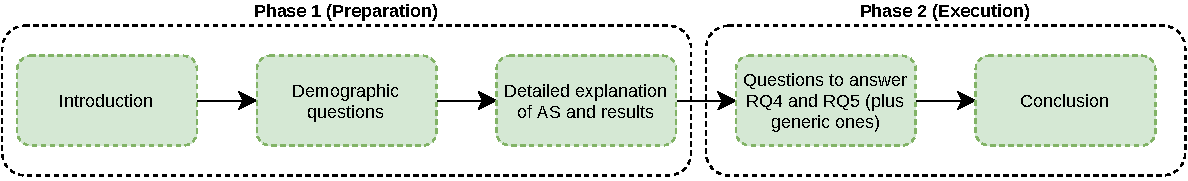
\includegraphics[width=0.8\textwidth]{c7/Fig4}
    \caption{Trade-offs between design-time and run-time quality attributes reported by the subjects. Edge weights represent the number of trade-offs.}\label{c7:fig:trade-offs} 
\end{figure}

One remarkable observation is that most subjects had difficulties identifying the trade-off decisions they made, especially in the case of implicit trade-offs. Additionally, some participants admitted that there may be trade-offs that they are not aware of yet; these are both implicit and inadvertent trade-offs and are very difficult to uncover. 

\subsection{RQ3 -- What processes, practices, and tools do ES practitioners follow to support trade-off decisions?}
The results indicate that no particular process (i.e. ATAM, AHP, QFD, ADD, etc. \cite{Barney2012}) is adopted when a decision that impacts both run-time and design-time qualities has to be taken.

The decision-making process in the cases studied follows common sense and normal intra-team interaction dynamics. Specifically, the following practices were common among the studied cases.
Since most of the projects studied are developed by small teams, it is common for software architects to also write code and work closely with other developers.
Most of the decisions that imply a trade-off between essential quality attributes are taken by the architects themselves, potentially in consultation with other team members.
However, when an important trade-off decision has to be made, the project leader is consulted in order to decide on how to proceed.
These cases usually concern the modification of a functionality that might be of interest for the customer of the project (e.g. a change in the requirements).
Most of the teams do not consult external experts, but one of the teams reported to occasionally do so, especially when dealing with complicated third-party libraries impacting the performance of their code.

The subjects support their trade-off decisions by acquiring input from different tools used to measure run-time metrics related to resource usage (i.e. CPU, network, memory) and test results. 
Specific tools are occasionally used, but the most common practice for measuring execution times, memory used, and network usage is logging.
Specific domain-related devices that are used as an important input are flight and hardware simulators.
Teams working on projects relying on cloud services for managing their back-end use the resource monitoring tools to pinpoint hot-spots and drive their decisions related to the code.
The study participants working in the HPC domain use an internal spreadsheet to estimate the performances of the card based on the clock frequency and the characteristics of the card design.
We emphasise that all aforementioned tools are used to measure \textit{individual} qualities; there were no subjects using dedicated tools that manage \textit{trade-offs} between qualities.

The findings can be summarised by stating that the study participants adopt a more lightweight and ad-hoc approach to deal with decisions rather than using a particular decision-support method.
By lightweight and ad-hoc we mean that they do not use specific methodologies, but they rather do an educated choice based on the data they have available, their own experience and of the other team members, and of course customer feedback whenever available.
The main reason is the limited amount of time between releases (or demos), which forces them to directly tackle the issues they are facing in the most rapid manner in order to continue the development of the system and deliver the product to the customer.

\subsection{RQ4 -- What would be the ideal features of a tool supporting quality attribute trade-off decisions?}
The features hereby are originated directly from the ideas of the focus group and interviewees participants, they range from very specific topics in trade-off management to the measurement of individual qualities.
The next subsections report on each category.

\subsubsection{Trade-off management}
Concerning features related to \textit{trade-off management}:
\begin{itemize}
    \item A common demand was the possibility to select a quality attribute for which the system should propose potential optimisations and highlight eventual trade-offs arising from applying them.
    For example, the envisioned system would propose changes that might improve the Maintainability level of a particular class, showing the possible impact on, for example, energy consumption for each proposed change.
    Similar analyses should also be supported for other quality attributes, such as Energy Efficiency and Security.
    The rationale behind this requirement is to help practitioners increase a certain quality of the system and, at the same time raise awareness about the impact on other quality attributes involved in the optimisation;

    \item The ability to register explicit trade-offs, especially in terms of accepting the compromised qualities, was also deemed important. For example, tools that perform continuous analysis of quality attributes, will keep issuing warnings related to the diminished quality (because of the trade-off). Practitioners mentioned that they would like to turn such warnings off since it would not make sense to address them: that would simply cancel the effects of the trade-off decision.
    For example, by simplifying the cognitive complexity of a method, thus easing maintainability, one might introduce energy inefficiencies.
    If this optimisation was suggested and effected by the tool, then one should be able to turn off the consequent energy warnings;

    \item Another interesting feature is the consequent impact of an applied optimisation on test coverage, or, more specifically, which tests have to be re-executed.
    The rationale behind this requirement is that executing tests is a time-consuming activity, thus, re-executing only tests affected by the applied change would greatly influence the productivity of the developers.
    
    \item Concerning Energy Efficiency, some practitioners would be interested to know what changes in the source code have a higher impact on the overall energy drawn by the system.
    This kind of feature can be applied at refactorings that focus on both improving Energy Efficiency and Maintainability, thus highlighting possible trade-offs between run-time and design-time qualities.   
\end{itemize}

\subsubsection{Technical project management}
Ideal features that relate to \textit{technical project management} are listed below:
\begin{itemize}
    \item An important feature is the possibility to set a user-defined severity level for each quality rule detected through static analysis, depending on the project being analysed, and on the software component where the issue is detected.
    The rationale behind this feature stems from the fact that different projects require different quality levels.
    In fact, the concept of quality often depends on the contract stipulated by the company and its customers.
    Hence, it is important to allow the user to define the desired level of quality for each project. For example, if the customer values Security, then security issues in critical components can be given very high severity;
    %So the user measures the risk of the project of not being accepted by the customer based on the quality attributes her customer desires;

    \item The practitioners also expressed their interest in monitoring the extended resource usage over a certain threshold defined by the user (e.g. software uses CPU over 85\% for more than 10 seconds).
    The rationale is that the user wants to ensure that there is a margin for a \textit{potential growth}\footnote{Note that this concept differs from Scalability for it is meant as an indefinite increase in the number of features that the system is able to offer.} of the system.
    In particular, reserving a certain margin of the available resources, such as memory or CPU time, for a potential future growth guarantees that the functionalities offered by a device can be increased without requiring hardware updates, thus extending the lifespan of the product.
    On top of this, it is especially important in critical embedded systems that, in case of malfunctioning, there are enough resources available to handle emergency situations.
    
    \item In some cases, the remote parts of some systems rely on 4G network connectivity to properly function. Practitioners working on these kind of projects have expressed the need of estimating the data usage of their system in order to have an idea of the (partial) cost of running the system. As the number of remote sensors with embedded sim cards in the system increases, every bit exchanged by a sensor has a higher impact on the final cost generated by the system.
    
\end{itemize}

\subsubsection{Monitoring quality attributes}
The features related to \textit{monitoring quality attributes}:
\begin{itemize}
    \item Resource profiling (CPU, memory, disk, etc.) seemed to be very popular since practitioners consider the quantification of run-time qualities (e.g. Reliability, Performance, or Energy Efficiency) of interest to be of paramount importance;
    
    \item In relation with Energy Efficiency, an interesting but hard-to-satisfy need is the automatic detection of possible optimisations of sensors and hardware usage by the software.
    One example could be the number of frames per second registered by a camera, which in case it is excessive and unneeded, it negatively influences energy consumption;
    
    \item Technical debt monitoring is also appealing to some of the practitioners.
    In particular, they deemed very useful to break down the overall technical debt by associating specific technical debt items to individual software components; this, in turn, helps to to better focus maintenance efforts.
\end{itemize}

Finally, there were also other, more generic features, such as security vulnerability identification, bug detection, and weekly reports on design-time and run-time qualities evolution.

\section{Discussion}\label{c7:sec:discussion}
This study investigated how software engineers and architects, from different companies from the embedded systems domain, prioritise and manage quality attributes, (paying special attention to \textit{Maintainability}, \textit{Dependability}, and \textit{Energy Efficiency}) and the trade-offs among them.

The results from RQ1 indicate that the involved practitioners focus their development efforts mostly on Dependability (more specifically, on \textit{Availability} and \textit{Reliability}). Although they value Maintainability as a top-priority quality attribute (as also identified by Bellomo et al. \cite{Bellomo2015}), they fail to effectively measure and monitor it with dedicated tools.
Several factors could cause this behaviour:
\begin{itemize}
    \item practitioners often lack theoretical knowledge on how the tools calculate metrics, what these metrics mean and how the metrics can be customised to better fit their context. In addition they usually do not have enough insight into the available tools (commercial or open-source) to be able to select the one that fits them better;

    \item most projects have very short iterations that require developers to focus on implementing functionality, while maintainability is not prioritised with the reasoning of not having business value;

    \item practitioners often have a short-term perspective on a specific project e.g. due to changing projects frequently. Thus the long-term sustainability of a project is not an immediate concern for them;
    
    \item the contract with the customer often does not explicitly concern architecture or code quality, thus the company might not invest on it;
    
    \item and finally, due to lack of training or company culture, developers may misunderstand or underestimate the shortcomings in maintainability.

\end{itemize}
%Given all these possibilities, it is hard to actually identify the common cause (if it actually exists) for not assessing the design and code quality of their systems with the aid of advanced automated tooling.

The majority of the trade-off experiences mentioned by the subjects (reported in RQ2) involve Maintainability as the compromised quality attribute whereas Dependability or Performance are favoured in most of the cases.
This finding aligns with what has been already reported by two other studies from the investigated literature \cite{Ampatzoglou2016,Feitosa2015}.
It is worth mentioning that the results of the three studies (this study, \cite{Ampatzoglou2016} and \cite{Feitosa2015}) were obtained in different contexts, using different data collection methodologies and data sources, while the similarities among them appear to be particularly strong. Therefore, these results seem to generalise well increasing the external validity of the studies.

Regarding the explicit or implicit nature of trade-offs reported in RQ3, the results from RQ2 indicate that the majority of the trade-offs can be considered explicit.
Through this observation alone, we could derive the conclusion that practitioners are perfectly aware of almost all the trade-offs they make and the qualities involved; yet, this would be a skewed view of reality caused by \textit{survivorship bias}. That is because practitioners \textit{do not thoroughly} monitor most of the design-time quality attributes -- as emerges from RQ1 -- and implicit trade-offs are harder to remember and report.
Hence, we conjecture that a significant amount of decisions entail \textit{implicit} trade-offs; especially those that incur technical debt due to un-monitored quality attributes, such as Maintainability.
As a result, the consequences of these implicit trade-offs are usually only discovered when new functionality, or performance optimisations, are required to be implemented, causing the developers to pay \textit{technical debt interest} on that part of the code.
The trade-off number one reported by RQ2 is a clear example of this phenomenon.

Another common practice that frequently causes practitioners to incur technical debt is the preparation for a demo. 
In general, this practice can be seen as incurring deliberate, but prudent, technical debt \cite{Fowler2014}, since it is a conscious decision made by the team in order to obtain a short-term advantage. 
One of the reasons that we deem this as `prudent', rather than `reckless' \cite{Fowler2014}, is because practitioners foresee very little interest probability on the parts of the system they rush before the demo; a possible explanation for this behaviour could be that customers might require a change involving that part of the system, so it might not be worth at all spending too much time on it.
This is reasonable since practitioners are required first and foremost to pursue customer satisfaction, rather than the long-term sustainability of source code. However, there needs to be a concrete strategy, after the demo, to monitor the incurred technical debt and strive to repay it as soon as possible.

Considering the results obtained from RQ3, it is reasonable to wonder why the subjects of the study do not use any specific process to support their trade-off decisions.
One possible explanation could be that, like most software engineering processes, those for managing trade-offs are not as well-known in industrial practice as in the academic domain.
Even if practitioners are familiar with such processes, many of them require a non-trivial amount of time to learn, plan, and eventually execute.
In particular, the planning and execution overhead are rather incompatible with the \textit{daily} routine of a developer and strict deadlines that characterise the industrial software domain, and, more specifically, the projects in our study. 
Note that since implicit trade-offs can arise from any decision taken, it could be necessary, depending on the case, to apply these methods on a daily basis.
Moreover, some of these processes involve multiple parties and project stakeholders, thus requiring substantial effort and calendar time to apply these methods for each decision; this does not align with teams following an agile software development process.
Also, a considerable amount of information concerning the system is usually required, which may not always be available in a practical amount of time, at the moment of making the decision.

An interesting aspect that emerges from the results is the prioritisation in managing trade-offs. Pipelining every decision through a trade-off decision-support process would add an excessive overhead; that would be counter-productive both on the short and on the long-term.
The only reasonable approach to manage trade-offs is to rationally select decisions that require support based on the foreseeable impact they have on the quality attributes of interest in the project, as well as potential risks. 
However, this is easier said than done.
Consider, for example, the fourth trade-off experience uncovered by RQ2, where engineers could have applied a trade-off decision-making support process to avoid heavily compromising on Maintainability and identify a new, more adequate, system architecture. 
They realised that cutting corners (i.e. bypassing layers) is the easiest way to improve performance, and did not bother considering eventual trade-offs since they were able to gain \textit{huge} performance improvements.
These large gains were enough of a reason for them to ignore long-term trade-offs, tackle their issue, and keep developing the system.

The abovementioned considerations can be generalised to companies that develop B2B (Business to Business) embedded system products that are meant to be sold to customers later on as personalised solutions.
The development of these products is done by teams that are small or medium sized (from 3-4 elements up to 6-7) and which members work closely together, perhaps covering multiple roles and wearing different hats depending on the development phase.
Embedded systems industry is forced by the market to move fast and innovate quickly, this requires their teams to react quickly to changes. 
In this regard, smaller teams of 3-5 members have been found to be the sweet spot for productivity in relation to the actual effort spent with a maximum of 9 elements by Putnam \cite{Putnam1978}. 
Moreover, teams with less than 10 elements are also the most frequent teams in software development \cite{Rodriguez2012}.

Finally, we summarise some of the implications of our study for practitioners and researchers.
Researchers now have a clearer view of the embedded systems industry's needs, practices, tools, quality attributes and trade-offs experiences, that can be used as a foundation for future research or experimental tool development. 
Furthermore, those interested in the practical aspects of technical debt management, now have a better insight on common habits and decisions concerning incurring technical debt (e.g. trade-offs and other practices from RQ2 and RQ3) and repaying technical debt (e.g. right after a demo, when there are less uncertainties and more time).
Also, they have now more insights on implicit and explicit trade-offs, which have not been studied before in the literature.
Practitioners on the other hand, can learn a lot from the reported experiences and the conclusions drawn by this study in order to further improve their development processes. 
For example, important decisions that involve quality attribute trade-offs should be supported by adequate decision-making processes or practices that document the qualities involved, keeping track of the decisions (e.g. using approaches proposed by other authors \cite{Heesch2012,Falessi2011,Barney2012}) and the favoured and sacrificed qualities.
Such documents can be subsequently used to support future decisions.
They can also become more aware of the importance to constantly monitor design-time quality attributes using dedicated software (i.e. that monitors technical debt, like SonarQube) and make trade-offs explicit, to the best possible extent.

\section{Threats to validity}\label{c7:sec:threats}
The present study is subject to limitations which can be categorised into \textit{construct validity}, \textit{external validity}, and \textit{reliability} following the classification proposed by Runeson et al. \cite{Runeson2012}.
Internal validity is not a concern for this study because we did not examine causal relations \cite{Runeson2012}.

\subsection{Construct validity}
Construct validity concerns the degree to which a study measures what it claims to be measuring \cite{Runeson2012}.

This study aimed at eliciting the knowledge of the practitioners in relation to a specific goal, expressed as research questions.
A case study protocol was carefully designed to ensure that the questions of the interviews and of the focus group were congruous with such a goal.
Additionally, the protocol was reviewed by an external reviewer to ascertain that indeed the data to be collected pertain to the research questions.

A possible construct validity threat comes from the risk that not all participants shared the same theoretical and technical knowledge of the high-level concepts covered during the interviews.
To address this threat, the interviewer ensured that each interviewee was on the same track as the others about the meaning of the main technical terms used throughout the interview by performing a brief explanation before using any of those terms.
The focus group participants received a similar explanation both in written form, prior to the session, and verbally, during the session.
Moreover, two pilot interviews were performed, and continuous feedback from the interviewed practitioners contributed to improving the clarity and the scope of the questions asked in the remaining interviews.
To avoid collecting data unrelated to the initial goal, the interviewees were required to discuss only projects respecting the criteria mentioned in Section \ref{c7:sec:interviews}. 
Finally, the possible bias introduced by the two participants that took part in both interviews and focus group was mitigated in two ways: first, the semi-structured format of the focus group was driven by a pre-defined agenda and we ensured no participant would cause us to deviate from that agenda; second, the session was moderated by an experienced researcher who intervened whenever necessary. Thus, given these two factors, the two participants could not mention or make reference to any  detail related to the interview that was yet not disclosed to the whole group.


\subsection{External validity}
External validity concerns whether the results of the study are generalisable to other similar environments, so that the results obtained are useful in other contexts.
There are two possible generalisations viewpoints: concerning the subjects and concerning embedded system fields.

Concerning the subjects, our study is based on data collected from several engineers coming from multiple companies. 
The engineers have a different field of specialisation and background, and their experience ranges from junior developers to very experienced system architects (see Tables \ref{c7:tab:iw-participants-background} and \ref{c7:tab:fg-participants-background}).
This variety of experiences covers a broad spectrum of embedded systems engineers, thus representing, at least to some extent,  the needs, the practices, and the tools used by practitioners working in the embedded systems domain.

Concerning the teams, the data collected by this study is mostly focused on small to medium software development teams.
This limitation slightly reduces the generalisations of the results, mostly from RQ3, to teams of similar sizes.
However, teams with less than 10 members are the most common teams in software development, regardless of the main programming language (and thus platform) used \cite{Rodriguez2012}, allowing these results to be applied to most teams.

Concerning the fields, this work discusses embedded systems that value Dependability, Performance, and Energy efficiency since most of the systems investigated perform tasks that are \textit{critical}, \textit{time-bounded}, or \textit{extended in duration} on devices relying on batteries.
The generalisation is however limited to companies that create systems meant for other businesses rather than to the average consumer.
Although these kinds of systems are only a small sample of the overall embedded systems population, the results obtained might be generalised to other domains that share a similar set of important quality attributes, such as industrial automation devices (Safety and Energy Efficiency), networking (Availability and Reliability), and scientific and measuring tools (high Performance).
However, one could argue that the study is unbalanced towards the aviation domain, since most of our subjects come from such a domain.
Nevertheless, several quality attributes that are critical in this domain are also critical in other domains considered; for example, Safety and Reliability are crucial attributes both in the Automotive and in the Medical implants fields.
Additionally, we considered each company as an individual case study subject, thus each company's needs were weighted according to the case study design, independently of the number of units of analysis they supplied for the study.

We cannot claim that the results can be generalised to other embedded system types, such as general consumer electronics, or machine learning applications, because different qualities or device types are preferred in these fields.

\subsection{Reliability}
Reliability, in this context, refers to the degree to which the collected data depends on the specific researchers collecting and analysing it (different researchers following the same case study design should yield the same data).
To this end, a replication package, containing the protocol and the questionnaires, is available online\footnote{Visit \url{http://www.cs.rug.nl/search/uploads/People/repl-package-ds18.zip}. }, allowing other researchers to evaluate the rigor of the design or replicate the study.

To guarantee the reliability of the findings, all the intermediary results were reviewed by a second researcher during all the process of analysis and the analysis was performed following a well-known qualitative data analysis method, namely Constant Comparative Method \cite{Boeije2002}. 
Additionally, the results were presented in front of at least one practitioner of each company that took part in the study in order to ensure that the sources of the data agree with the findings of the study and ensure their credibility.

\section{Conclusions}\label{c7:sec:conclusion}
Managing quality attribute trade-offs is a complicated activity that has a considerable impact on the system's behaviour and future sustainability.
The embedded systems domain is generally more sensitive to trade-offs among quality attributes than other domains since they have strict requirements on performance, energy and dependability.
For example, small changes to the design or code of the system might have an undesired impact on its run-time qualities.

By analyzing and understanding how the industry deals with trade-offs on a day-by-day basis, it is possible to propose solutions that support the industry in addressing this complicated problem.
To this end, this work investigated the needs and practices of the embedded systems industry on quality attribute trade-offs by directly interacting with a number of practitioners through interviews and a focus group.

A major finding from this study is that embedded systems engineers are in great need for tooling that supports the monitoring of run-time qualities, but at the same time indicates possible implications on design-time qualities of the performed changes.
Also, we found that practitioners rarely adopt tools for monitoring design-time quality attributes; this behaviour causes them to overlook important trade-offs that negatively impact the cost of the project in the long-term (i.e. incur technical debt).
Moreover, due to strict domain requirements, practitioners have difficulties applying methods, or processes, for explicitly managing trade-offs among quality attributes. Thus, they focus on the major run-time qualities, such as Dependability or Performance, that satisfy customer needs.

As future research perspective, it would be interesting to investigate the actual costs of trade-offs in a project and compare estimations of technical debt interest for implicit and explicit trade-offs.
Another interesting work would be to investigate an empirically-calculated ratio of explicit versus implicit trade-offs, allowing one to grossly estimate the hidden technical debt principal of a project using data of past decisions.

\section*{Acknowledgements}
Special thanks to Apostolos Ampatzoglou for providing suggestions and comments on the design of this study.
We would also like to thank all the companies that took part in this study and provided us with valuable information.